\documentclass[a4paper, 12pt, final, garamond]{book}
\usepackage{cours-preambule}

\makeatletter
\renewcommand{\@chapapp}{M\'ecanique -- chapitres}
\makeatother

\hfuzz=5.002pt

% \toggletrue{student}
% \toggletrue{corrige}
% \renewcommand{\mycol}{black}
\renewcommand{\mycol}{gray}

\begin{document}
\setcounter{chapter}{7}

% \settype{enon}
% \settype{solu_prof}
% \settype{solu_stud}

\chapter{\cswitch{Correction du TD}{TD~: m\'ecanique du solide}}

\resetQ
\section{Levier}
\enonce{%
	\textsc{Archimède} (240 av. J.-C.) est le premier à établir la théorie physique
	du levier et de la balance. Il aurait dit\ftn{Voir
		\url{https://www.persee.fr/doc/antiq_0770-2817_1955_num_24_1_3257} pour une
		restitution plus fidèle}~:
	\begin{quote}
		\openquote
		Donnez-moi un point fixe et un levier, et le soulèverai la Terre.\closequote
	\end{quote}
	Imaginons une situation pour réaliste où \textsc{Archimède} utilise un levier
	afin de soulever un rocher de masse $M = \SI{200}{kg}$. Les longueurs sont $d_1
		= \SI{50}{cm}$, $d_2 = \SI{1.5}{m}$ et $\alpha = \ang{60}$.
	\begin{figure}[htbp!]
		\centering
		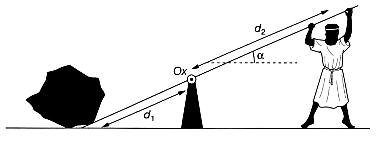
\includegraphics[width=.7\linewidth]{archi_plain-white}
		\label{fig:bld_1}
	\end{figure}
}

\QR{%
	\textsc{Archimède} se suspend verticalement au levier. Quelle doit être sa
	masse minimale pour que le rocher se soulève~?
}{%
	On fait un schéma et on détermine les distances des bras de levier pour
	calculer les moments~:
	\noindent
	\begin{minipage}[c]{.45\linewidth}
		\begin{align*}
			\Mc_x(\Pf_1) & = +\ell_1 m_1g = m_1d_1g \cos(\alpha)
			\\
			\Mc_x(\Pf_2) & = -\ell_2 m_2g = -m_2d_2g \cos(\alpha)
		\end{align*}
		Pour avoir rotation, il faut que le moment total soit \textbf{négatif} (sens
		horaire autour de (O$x$)), soit
	\end{minipage}
	\hfill
	\begin{minipage}[c]{.55\linewidth}
		~
		\begin{center}
			\includegraphics[width=\linewidth]{archi_levier-a}
		\end{center}
	\end{minipage}
	\begin{align*}
		\underbracket[1pt]{\cancel{g \cos(\alpha)}}_{\neq 0} \left( m_1d_1 - m_2d_2
		\right)    & < 0
		\\\Lra
		m_2d_2     & > m_1d_1
		\\\Lra
		\Aboxed{m_2 > m_1 \frac{d_1}{d_2}}
		\qav
		\left\{
		\begin{array}{rcl}
			m_1 & = & \SI{200}{kg}
			\\
			d_1 & = & \SI{0.50}{m}
			\\
			d_2 & = & \SI{1.5}{m}
		\end{array}
		\right.                    \\
		\makebox[0pt][l]{$\phantom{\AN}\xul{\phantom{m_{2,\min} = \SI{67}{kg}}}$}
		\AN
		m_{2,\min} & = \SI{67}{kg}
	\end{align*}
}
\QR{%
	\textsc{Archimède} décide de faire varier la direction de la force qu'il
	exerce sur le levier sans changer sa norme. Comment doit-il procéder pour être
	le plus efficace~? Quel est le gain par rapport au cas précédent~?
}{%
	On fait un schéma et on détermine les distances des bras de levier pour
	calculer les moments~:
	\noindent
	\begin{minipage}[c]{.45\linewidth}
		En modifiant la direction de la force, donc de la droite d'action, la
		longueur du bras de levier est modifiée~: on a, au mieux, $\boxed{\ell_2 =
				d_2}$, obtenu pour une force perpendiculaire au levier.
	\end{minipage}
	\hfill
	\begin{minipage}[c]{.55\linewidth}
		~
		\begin{center}
			\includegraphics[width=\linewidth]{archi_levier-b}
		\end{center}
	\end{minipage}
	\begin{DispWithArrows*}
		\sum_i \Mc_x(\Ff_i)    & < 0
		\Arrow{$\norm{\Ff_2} = m_2g$}
		\\\Lra
		m_1 \cancel{g} d_1 \cos(\alpha) - m_2 \cancel{g} d_2 &< 0
		\\\Lra
		\Aboxed{m_2 &> m_1 \frac{d_1}{d_2} \cos(\alpha)}
		\\
		\makebox[0pt][l]{$\phantom{\AN}\xul{\phantom{m_{2,\min} = \SI{33}{kg}}}$}
		\AN
		m_{2,\min} & = \SI{33}{kg}
	\end{DispWithArrows*}
	Autrement dit, avec $g = \SI{10}{m.s^{-2}}$, c'est \SI{330}{N} de force gagné
	par rapport à la situation précédente, soit un gain de 50\%~!
	\begin{tcb}(ror){À retenir}
		\begin{itemize}
			\item Dessinez les moments et les bras de levier des forces \textbf{et} indiquez
			      la direction de rotation induite par la force.
			\item Le moment total est la somme des moments
		\end{itemize}
	\end{tcb}
}

\resetQ
\section{Pendule pesant non amorti}
\enonce{%
	\noindent
	\begin{minipage}[c]{.70\linewidth}
		Une benne de téléphérique, de masse $M = \SI{2.0e3}{kg}$, est accrochée au point
		A situé à l'extrémité inférieure d'un bras de masse $m = \SI{300}{kg}$ relié à
		des câbles au point O. On note $d = \SI{4.5}{m}$ la distance entre O et G le
		centre de gravité de l'ensemble \{benne+bras\}, situé sur l'axe (OA).
	\end{minipage}
	\hfill
	\begin{minipage}[c]{.29\linewidth}
		~
		\begin{center}
			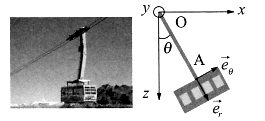
\includegraphics[width=\linewidth]{cabine_plain-white}
			\label{fig:cab_plain}
		\end{center}
	\end{minipage}
	On note $J\ind{tot}$ le moment d'inertie de l'ensemble par rapport à l'axe de
	rotation $y$, et la liaison est supposée parfaite. On effectue un test
	d'oscillations de la benne, le point O étant maintenant fixe.
}
\QR{%
	En appliquant le théorème du moment cinétique, déterminer l'équation
	différentielle vérifiée par $\th$.
}{%
	\begin{minipage}[c]{0.70\linewidth}
		\begin{itemize}
			\bitem{Système}~: \{benne+bras\} solide de masse $m\ind{tot} = m + M$
			\bitem{Référentiel}~: terrestre, supposé galiléen.
			\bitem{Repère}~:
			cylindrique $(\Or,\er,\et,\ey)$ avec O centre de la liaison pivot.
			\bitem{Repérage}~:
			\begin{empheq}[left=\empheqlbrace]{align*}
				\OG &= d\er\\
				\vf(\Gr) &= d \tp\et\\
				\af(\Gr) &= d \tpp \et - d \tp^2 \er
			\end{empheq}
		\end{itemize}
	\end{minipage}
	\hfill
	\begin{minipage}[c]{0.30\linewidth}
		\begin{center}
			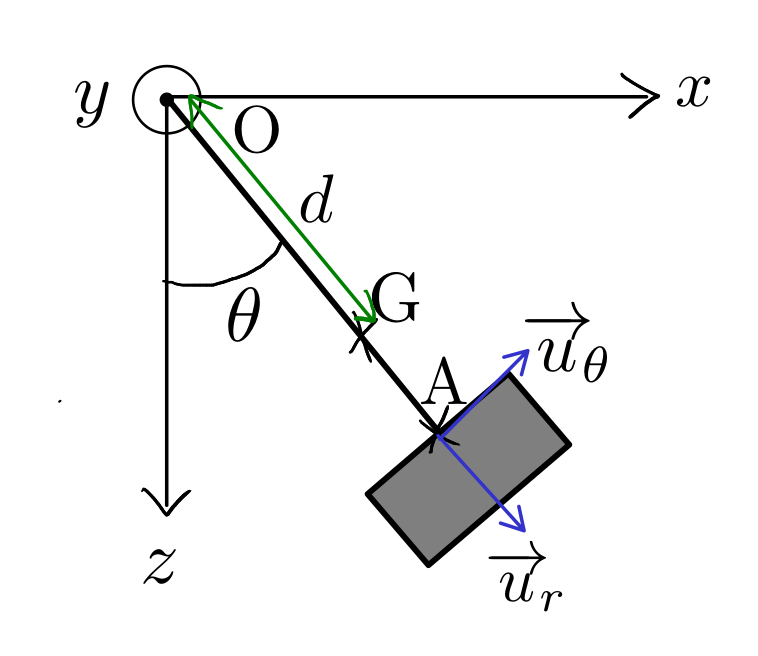
\includegraphics[width=\linewidth]{cabine_corr}
		\end{center}
	\end{minipage}
	\begin{itemize}
		\bitem{Bilan des forces}~:
		\begin{itemize}
			\item $\Pf = m \ind{tot}g \ey = m \ind{tot}g (\cos(\th)\er -
				      \sin(\th)\ut)$
			\item $\Ff = \of$ car pivot parfaite
		\end{itemize}
		\bitem{Bilan des moments}~:
		\begin{itemize}
			\item $
				      \Mcf_{\Or}(\Pf) =
				      \OG \wedge \Pf =
				      (d \er) \wedge (m \ind{tot}g (\cos(\th)\er - \sin(\th)\et))
				      \Lra
				      \boxed{\Mcf_{\Or}(\Pf) = -m \ind{tot}gd \sin(\th)\ey}$
			      \smallbreak
			      Par projection, on retrouve le résultat qu'on aurait eu avec le bras
			      de levier~:
			      \[
				      \ell = d \sin(\th) \qet \norm{\Pf} = m \ind{tot}g
				      \quad \Ra \quad
				      \boxed{\Mc_y (\Pf) = - m \ind{tot}g d \sin(\th)}
			      \]
			\item $\Lc_y(\Sc) = J\ind{tot} \tp$
		\end{itemize}
		\bitem{TMC}~:
		\vspace{-20pt}
		\[
			\dv{\Lc_y (\Sc)}{t} = \Mc_y(\Pf)
			\Lra
			J\ind{tot} \tpp = -m \ind{tot}g d \sin(\th)
			\Lra
			\boxed{\tpp + \frac{m \ind{tot}gd}{J\ind{tot}} \sin(\th) = 0}
		\]
	\end{itemize}
}
\QR{%
	En déduire la période $T$ des petites oscillations de la benne.
}{%
	Petites oscillations $\Ra \sin(\th) \Sim_{\th \to 0} \th$, donc oscillateur
	harmonique~:
	\[
		\w_0 = \sqrt{\frac{m \ind{tot}gd}{J\ind{tot}}}
		\Lra
		\boxed{T = 2\pi\sqrt{\frac{J\ind{tot}}{m \ind{tot}gd}}}
	\]
}
\QR{%
	Sachant que la période des petites oscillations est $T = \SI{4.1}{s}$ et que
	le bras de longueur $L = \SI{3.0}{m}$ a un moment d'inertie $J' =
		\frac{1}{3}mL^2$ par rapport à l'axe $y$, calculer le moment d'inertie $J$ de
	la benne par rapport à $y$. On rappelle que $g = \SI{9.81}{m.s^{-2}}$ et on
	indique que dans ce cas, les moments d'inertie se somment.
}{%
	En restant autour du même axe, les moments cinétiques se somment, soit
	$J\ind{tot} = J\ind{bras} + J\ind{benne}$. On isole $J\ind{tot}$~:
	\begin{align*}
		J\ind{tot} & = \frac{T^2}{4\pi^2} m \ind{tot} gd
		\\\Lra
		J          & = \frac{T^2}{4\pi^2} m \ind{tot}gd - J'
		\\\Lra
		\Aboxed{J  & = \frac{T^2}{4\pi^2} m \ind{tot}gd - \frac{mL^2}{3}}
		\qav
		\raisebox{0pt}[0pt][0pt]{$
				\left\{
				\begin{array}{rcl}
					T           & = & \SI{4.1}{s}
					\\
					L           & = & \SI{3.0}{m}
					\\
					d           & = & \SI{4.5}{m}
					\\
					m           & = & \SI{300}{kg}
					\\
					m \ind{tot} & = & \SI{2.3e3}{kg}
					\\
					g           & = & \SI{9.81}{m.s^{-2}}
				\end{array}
				\right.$
		}                                                                 \\
		\makebox[0pt][l]{$\phantom{\AN}\xul{\phantom{J = \SI{6.8e7}{kg.m^2}}}$}
		\AN
		J          & = \SI{4.2e4}{kg.m^2}
	\end{align*}
}

\resetQ
\section{Chute d'un arbre}
\enonce{%
	\noindent
	\begin{minipage}[t]{.78\linewidth}
		On étudie la chute d'une arbre~: on souhaite connaître la durée que met l'arbre,
		une fois tranché à sa base, pour tomber au sol.
		\smallbreak
		On modélise la situation par une tige homogène de hauteur $L = \SI{10}{m}$ et de
		masse $m$, reliée au sol par une liaison pivot parfaite et qui part d'un angle
		initial $\th_0 = \SI{1.5}{rad}$ avec une vitesse initiale nulle. On donne le
		moment d'inertie par rapport à O$z$~: $J_z = \frac{1}{3}mL^2$.
	\end{minipage}
	\hfill
	\begin{minipage}[t]{.20\linewidth}
		~
		\begin{center}
			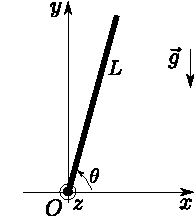
\includegraphics[width=\linewidth]{arbre_plain.pdf}
			\label{fig:arbre_chute}
		\end{center}
	\end{minipage}
}

\QR{%
	Donner les expressions des énergies cinétique et potentielle de pesanteur de
	l'arbre.
}{%
	\noindent
	\begin{minipage}[t]{.45\linewidth}
		\begin{gather}
			\notag
			\Ec_c = \frac{1}{2}J \tp^2
			\qet
			\Ec_{p,p} = mgy_{\Gr} + 0
			\\
			\notag
			\beforetext{Or}
			y_{\Gr} = \frac{L}{2}\sin(\th) \Ra \Ec_{p,p} = \frac{mgL}{2}\sin(\th)
			\\\Ra
			\boxed{\Ec_m = \frac{1}{2}J \tp^2 + \frac{mgL}{2}\sin(\th)}
			\label{eq:arbre_1}
		\end{gather}
	\end{minipage}
	\hfill
	\begin{minipage}[t]{.30\linewidth}
		\vspace{0pt}
		\begin{center}
			\includegraphics[width=\linewidth]{arbre_corr}
		\end{center}
	\end{minipage}
}
\QR{%
	Justifier que l'énergie mécanique est constante au cours du mouvement.
	Exprimer cette constante en utilisant les conditions initiales.
}{%
	Le système n'est soumis qu'à son poids, conservatif, et à l'action de la
	liaison pivot, supposée parfaite donc sans frottement. Le système est donc
	conservatif, et par TPM on a $\dv{\Ec_m}{t} = 0$.
	\smallbreak
	On a donc $\Ec_m(t) = \Ec_{m}(0)$, or $\Ec_c(0) = 0$ et $\Ec_{p,p}(0) =
		\frac{mgL}{2}\sin(\th_0)$, soit
	\begin{equation}
		\Ec_m = \frac{mgL}{2}\sin(\th_0)
		\label{eq:arbre_2}
	\end{equation}
}
\QR{%
	En déduire la relation
	$\DS \dv{\th}{t} = - \sqrt{\frac{3g}{L}(\sin{\th_0} - \sin{\th})}$
}{%
	\vspace{-20pt}
	\begin{align*}
		\eqref{eq:arbre_1}                        & = \eqref{eq:arbre_2}
		\\\Lra
		\frac{1}{2}J \left( \dv{\th}{t} \right)^2 & =
		\frac{mgL}{2} \left( \sin(\th_0) - \sin(\th) \right)
		\\\Lra
		\left( \dv{\th}{t} \right)^2              & =
		\frac{3mgL}{mL^2} \left( \sin(\th_0) - \sin(\th) \right)
		\\\Ra
		\dv{\th}{t}                               & = \pm
		\sqrt{\frac{3g}{L}\left( \sin(\th_0) - \sin(\th) \right)}
		\intertext{Or, de toute évidence $\th$ \textbf{diminue} puisque l'arbre
			tombe ($\Mc_z(\Pf) < 0$), soit}
		\Aboxed{\dv{\th}{t}                       & =
			- \sqrt{\frac{3g}{L}\left( \sin(\th_0) - \sin(\th) \right)}}
		\qed
	\end{align*}
}
\QR{%
	Retrouver ce résultat par le TMC.
}{%
	Avec le bras de levier, on a $\DS \Mc_z(\Pf) = - \frac{mgL}{2}\cos(\th)$.
	Ainsi, avec le TMC,
	\begin{DispWithArrows*}
		\dv{\Lc_z}{t} &= \Mc_z(\Pf)
		\\\Lra
		J \tpp &= - \frac{mgL}{2}\cos(\th)
		\CArrow{$\times \tp$}
		\\\Lra
		J \tpp \tp &= - \frac{mgL}{2}\cos(\th) \tp
		\CArrow{$\int (\cdot) \dd{t}$}
		\\\Ra
		J \int_{t=0}^{t}
		\frac{\dd}{\cancel{\dd{t}}}\pac{\frac{1}{2}\tp^2}\cancel{\dd{t}} &=
		- \frac{mgL}{2}\int_{t=0}^{t}
		\cos(\th)\frac{\dd{\th}}{\cancel{\dd{t}}}\cancel{\dd{t}}
		\Arrow{$\int \cos(\th)\dd{\th} = \int \dd{\pac{\sin(\th)}}$}
		\\\Lra
		\tp^2(t) - \underbracket[1pt]{\cancel{\tp^2(0)}}_{=0} &=
		- \frac{mgL}{2J} \pa{\sin(\th) - \sin(\th_0)}
		\Arrow{$J = \frac{mL^2}{3}$}
		\\\Lra
		\tp^2(t) &= - \frac{3 \cancel{m}g \bcancel{L}}{\cancel{m}L^{\bcancel{2}}}
		\pa{\sin(\th) - \sin(\th_0)}
		\Arrow{On prend l'opposé}
		\\\Lra
		\tp^2(t) &= \frac{3g}{L}\pa{\sin(\th_0) - \sin(\th)}
		\Arrow{$\dv{\th}{t} < 0$}
		\\\Ra
		\Aboxed{\dv{\th}{t} &= -
			\sqrt{\frac{3g}{L}\left( \sin(\th_0) - \sin(\th) \right)}}
		\qed
	\end{DispWithArrows*}
	On retiendra ici deux choses~:
	\begin{tcb}(ror){À retenir}
		\begin{itemize}
			\item Penser à multiplier par $\tp$ pour facilement intégrer les relations
			      avec $\tpp$ et des fonctions transcendantales (cos, sin…)
			\item Attention en prenant la racine carré d'une fonction~: toujours
			      écrire les deux valeurs possibles et vérifier la faisabilité
			      physiquement.
		\end{itemize}
	\end{tcb}
}
\QR{%
	Pour exprimer la durée $T$ de la chute, isoler $\dd{t}$ dans l'expression
	précédente puis l'intégrer entre $\th = \th_0$ et $\th = 0$. Faire
	l'application numérique, sachant que $\DS
		\int_{0}^{\th_0}\frac{\dd{\th}}{\sqrt{\sin{\th_0} - \sin{\th}}} \approx
		\num{5.44}$ pour $\th_0 = \SI{1.5}{rad}$.
}{%
	On inverse pour avoir
	\[
		\dd{t} = \frac{-\dd{\th}}{\sqrt{\frac{3g}{L}\pa{\sin(\th_0)-\sin(\th)}}}
	\]
	Or, quand $\eval{t}^{t_f}_0$, on a $\eval{\th}^{\th_f=0}_{\th_0}$. Ainsi,
	\begin{DispWithArrows*}[]
		\int_{0}^{t_f} \dd{t} &=
		\int_{\th_0}^{0} \frac{-\dd{\th}}{\sqrt{\frac{3g}{L}\pa{\sin(\th_0)-\sin(\th)}}}
		\Arrow{On inverse les bornes avec $-$}
		\\\Lra
		t_f - 0 &=
		\sqrt{\frac{L}{3g}} \int_{0}^{\th_0} \frac{\dd{\th}}{\sqrt{\sin(\th_0)-\sin(\th)}}
		\\
		\makebox[0pt][l]{$\phantom{\AN}\xul{\phantom{t_f = \SI{3.2}{s}}}$}
		\AN
		t_f &= \SI{3.2}{s}
	\end{DispWithArrows*}
}
\begin{pycode}
from scipy.integrate import quad  # Module d'intégration "quad"
import numpy as np

# Intervalle d'intégration
theta_0 = 1.5 # rad
theta_f = 0   # rad

# Constantes
L = 10               # m
g = 9.81             # m.s^-2
K = np.sqrt(L/(3*g)) # s

# Fonction à intégrer
def function(theta):
  return K/(np.sqrt(np.sin(theta_0) - np.sin(theta)))

# Calcul de l'intégrale
res, err = quad(function, theta_f, theta_0)

# Affichage du résultat
# print(f"Résultat de l'intégrale = {res:.2f} ± {err:.2f}")
\end{pycode}
\QR{%
	\textit{Bonus} Écrire un script \texttt{Python} permettant de calculer
	numériquement l'intégrale précédente.
}{%
	On obtient bien $t_f = \py{fr'\SI{{{res:.2f}}}{{s}}'}$ avec~:
\begin{tcb}(code)<lfnt>{Code}
\inputpygments[numbers=left,xleftmargin=10pt]{python}{TDM8_solide-arbre.py}
\end{tcb}
}

\resetQ
\section{Barre fixée à ses extrémités}
\enonce{%
	\noindent
	\begin{minipage}[c]{.70\linewidth}
		Considérons le système mécanique représenté ci-contre, constitué d'une barre
		homogène de masse $m$, de longueur OA $= 2a$, libre de tourner sans frottement
		autour de l'axe O$z$ (liaison parfaite). Son moment d'inertie par rapport à
		cet axe vaut $J_z = \frac{4}{3}ma^2$. Elle est attachée en A à un ressort de
		longueur à vide $\ell_0$ et de raideur $k$. L'autre extrémité du ressort est
		fixe.
	\end{minipage}
	\hfill
	\begin{minipage}[c]{.25\linewidth}
		\begin{center}
			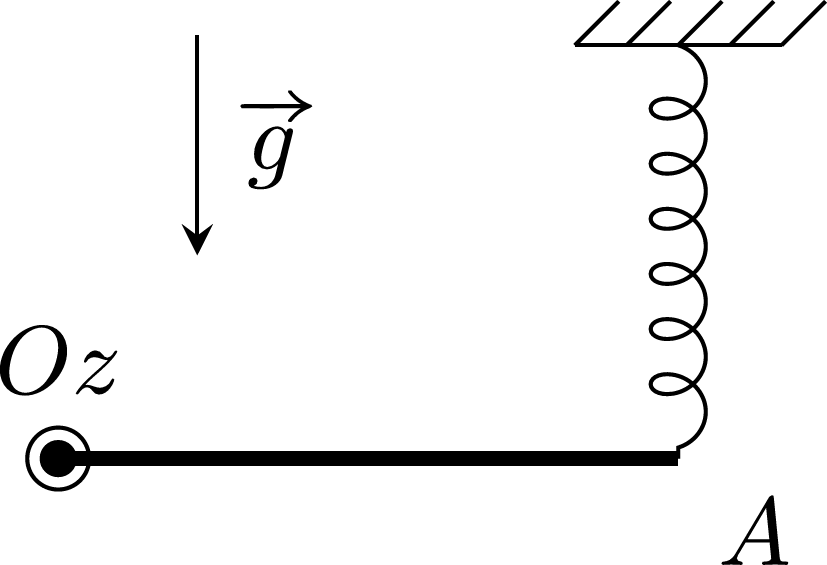
\includegraphics[width=\linewidth]{brr_fixe-plain}
		\end{center}
	\end{minipage}
}

\QR{%
	À l'équilibre, las barre est horizontale et le ressort vertical. En déduire la
	longueur du ressort à l'équilibre en fonction de $k, \ell_0, m$ et $g$.
}{%
	\noindent
	\begin{minipage}[t]{.70\linewidth}
		\begin{itemize}
			\bitem{Système}~: \{barre\}
			\bitem{Référentiel}~: terrestre supposé galiléen
			\bitem{Repère}~: $(\Or,\ux,\uy,\uz)$
			\bitem{Repérage}~: $\OG = a\ux$ et $\vvr{OA} = 2a\ux$
			\bitem{BdF}~: \textbf{à l'équilibre}, le ressort est vertical, soit
			\begin{itemize}
				\item $\Pf = -mg\uy$~;
				\item $\Ff_r = k(\ell\ind{eq} - \ell_0)\uy$.
				\item $\Ff_f = \of$ pas de frottements
			\end{itemize}
		\end{itemize}
	\end{minipage}
	\begin{minipage}[t]{.30\linewidth}
		\vspace{0pt}
		\begin{center}
			\includegraphics[width=\linewidth]{brr_fixe-corr.pdf}
		\end{center}
	\end{minipage}
	\begin{itemize}
		\bitem{BdM}~: avec les bras de levier, qui se confondent ici avec les
		distances des points d'application puisque les droites d'actions sont
		perpendiculaires à l'objet, on trouve
		\begin{itemize}
			\item $\Mc_z(\Pf) = -a \times mg$ (sens horaire)~;
			\item $\Mc_z(\Ff_r) = +2a \times k (\ell\ind{eq}-\ell_0)$.
			\item $\Mc_z(\Ff_f) = 0$ pivot parfaite.
		\end{itemize}
		\bitem{TMC}~: à l'équilibre, pas de rotation donc
		\[
			\Mc_z(\Pf) + \Mc_z(\Ff_r) = 0
			\quad \Lra \quad
			-mga + 2ak (\ell\ind{eq}-\ell_0) = 0
			\quad \Lra \quad
			\boxed{\ell\ind{eq} = \ell_0 + \frac{mg}{2k}}
		\]
	\end{itemize}
}
\QR{%
	La barre est légèrement écartée de sa position d'équilibre, puis lâchée sans
	vitesse initiale. Déterminer la période des petites oscillations. Comme les
	angles sont très petits, on peut considérer que le point A se déplace
	verticalement.
}{%
	\noindent
	\begin{minipage}[t]{.60\linewidth}
		Avec un angle, les droites d'actions ne sont plus
		perpendiculaires à la barre donc les bras de levier ne se confondent plus
		avec les distances des points d'application. Il faut refaire un schéma et
		recalculer les moments~:
	\end{minipage}
	\hfill
	\begin{minipage}[t]{.40\linewidth}
		\vspace{-20pt}
		\begin{center}
			\includegraphics[width=\linewidth]{brr_fixe-corr-b.pdf}
		\end{center}
	\end{minipage}
	\vspace{-20pt}
	\begin{itemize}
		\bitem{BdM}~:
		\begin{itemize}
			\item $\Mc_z(\Pf) = -a \cos(\th) \times mg$~;
			\item $\Mc_z(\Ff_r) = +2a \cos(\th) \times k (\ell - \ell_0)$
			      \smallbreak
			      Or, $\ell$ n'est plus $\ell\ind{eq}$ puisqu'on n'est plus à l'équilibre.
			      On trouve $\ell = \ell\ind{eq} - 2a \sin(\th)$, soit finalement
			      \[
				      \Mc_z(\Ff_r) =
				      +2a \cos(\th) \times k (\ell\ind{eq} - 2a\sin(\th) - \ell_0)
			      \]
			\item $\Lc_z = J_z\tp$
		\end{itemize}
		\bitem{TMC}~:
		\vspace{-20pt}
		\begin{DispWithArrows*}[groups]
			\dv{\Lc_z}{t} &= \sum_i \Mc_z(\Ff_i)
			\\\Lra
			J_z \tpp &=
			-a \cos(\th) \times mg +
			2a \cos(\th) \times k (\ell\ind{eq} - 2a\sin(\th) - \ell_0)
			\Arrow{$\cos(\th) \approx 1$\\$\sin(\th) \approx \th$}
			\\\Lra
			J_z \tpp &= -mga + 2ak(\ell\ind{eq} - 2a\th - \ell_0)
			\\\Lra
			J_z \tpp &= -mga - 4ak\th + 2ak (\ell\ind{eq}-\ell_0)
			\Arrow{$2ak (\ell\ind{eq} - \ell_0) = mga$}
			\\\Lra
			J_z \tpp &= \cancel{-mga} + \cancel{mga} - 4ak\th
			\Arrow{$J_z = \frac{4}{3}ma^2$}
			\\\Lra
			\Aboxed{\tpp + \frac{3k}{m}\th &= 0}
			\Arrow{$\w_0 = \sqrt{\frac{3k}{m}}$}
			\\\Ra
			\Aboxed{T_0 &= 2\pi \sqrt{\frac{k}{3}}}
			\qed
		\end{DispWithArrows*}
	\end{itemize}
}

\resetQ
\section{Choc de deux chariots}
\enonce{%
	\noindent
	\begin{minipage}[c]{.45\linewidth}
		Deux masses $m_1$ et $m_2$ sont montées sur un banc horizontal à coussins
		d'air, de sorte qu'on peut négliger tout frottements. On les projette l'une
		contre l'autre avec des vitesses initiales $\vf_1 = v_1 \ux$ et $\vf_2 =
			\of$ ($m_2$ initialement à l'arrêt).
	\end{minipage}
	\hfill
	\begin{minipage}[c]{.45\linewidth}
		~
		\begin{center}
			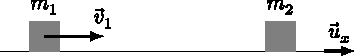
\includegraphics[width=\linewidth]{chariots-plain}
		\end{center}
	\end{minipage}
}

\begin{blocQR}
	\item \textit{Dans cette partie, on suppose qu'après le choc les masses
		restent solidaires.}
	\QR{%
		Quelle est la vitesse commune des deux masses après le choc~?
	}{%
		\begin{itemize}
			\bitem{Système}~: \{2 chariots\} considérés chacun comme un point matériel
			\bitem{Référentiel}~: terrestre supposé galiléen
			\bitem{Base}~: $(\ux,\uz)$ avec $\uz$ vertical ascendant
			\bitem{BdF}~:
			\begin{itemize}
				\item $\Pf_1 = -m_1g\uz$ et $\Nf_1 \uz$ pour le premier
				\item $\Pf_2 = -m_2g\uz$ et $\Nf_2 \uz$ pour le second
				\item Aucune force de frottements, donc système pseudo-isolé ($\sum_i
					      \Ff_i = \of$)
			\end{itemize}
		\end{itemize}
		\begin{center}
			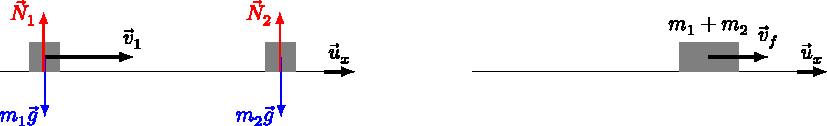
\includegraphics[width=\linewidth]{chariots-corr_a}
		\end{center}
		Ainsi, $\dv{\pf_{\tot}}{t} = \of$ soit $\pf_{\tot} = \vcte$. Ainsi,
		\[
			m_1\vf_1 + m_2\vf_2 = (m_1+m_2)\vf_f
			\quad \Lra \quad
			\boxed{\vf_f = \frac{m_1}{m_1+m_2}v_1\ux}
		\]
	}
	\QR{%
		Quel est le travail des actions intérieures lors du choc~? Commenter le
		signe du résultat.
	}{%
		On utilise le TEC~:
		\begin{gather*}
			\D{\Ec_{c}} = W\ind{int} + \underbracket[1pt]{W\ind{ext}}_{=0}
			\quad \Lra \quad
			W\ind{int} = \Ec_f - \Ec_i = \frac{1}{2}(m_1+m_2)v_f{}^2 -
			\frac{1}{2}m_1v_1{}^2
			\\\Lra
			\boxed{W\ind{int} = - \frac{m_1m_2}{2 (m_1+m_2)}v_1{}^2 < 0}
		\end{gather*}
		Le travail des forces intérieures est donc \textbf{négatif}, ce qui est
		cohérent avec le fait que le système perd de l'énergie cinétique,
		transformée en énergie thermique lors du choc.
	}
\end{blocQR}
\begin{blocQR}
	\item \textit{On considère dans cette partie que le choc est élastique,
		c'est-à-dire que l'énergie cinétique de l'ensemble des deux masses est
		conservée au cours du choc et qu'elles ne sont plus solidaires après.}
	\QR{%
		Montrer que les vitesses $v_1'$ et $v_2'$ après le choc s'expriment~:
		\[
			v_1' = \frac{m_1-m_2}{m_1+m_2}v_1
			\qet
			v_2' = \frac{2m_1}{m_1+m_2}v_1
		\]
	}{%
		On a toujours un système pseudo-isolé~:
		\begin{center}
			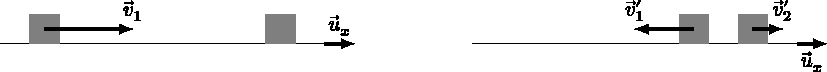
\includegraphics[width=\linewidth]{chariots-corr_b}
		\end{center}
		On a donc la conservation de la quantité de mouvement totale, ainsi que
		l'énergie cinétique totale~; ainsi entre les deux situations~:
		\begin{gather*}
			\left\{
			\begin{array}{rl}
				m_1v_1                & = m_1v_1' + m_2v_2'
				\\
				\frac{1}{2}m_1v_1{}^2 & = \frac{1}{2}m_1v_1' + \frac{1}{2}m_2v_2'
			\end{array}
			\right.
			\Lra
			\boxed{
				\left\{
				\begin{array}{rl}
					v_1' & = \DS \frac{m_1-m_2}{m_1+m_2}v_1
					\\
					v_2' & = \DS \frac{2m_1}{m_1+m_2}v_1
				\end{array}
				\right.}
		\end{gather*}
	}
	\QR{%
		Que se passe-t-il si $m_2 \gg m_1$~?
	}{%
		Si $m_2 \gg m_1$, alors $v_1' \to -v_1$ et $v_2' \to 0$. La masse $m_1$
		rebondit sur la masse $m_2$, qui elle reste immobile. C'est la situation du
		lancer d'une balle rebondissante sur un mur.
	}
	\QR{%
		À quelle condition sur $m_1$ et $m_2$ est-il possible de réaliser un
		«~carreau~», i.e.\ échanger lors du choc les vitesses des deux masses,
		comme à la pétanque~?
	}{%
		Pour faire un carreau, on veut $v_1' = 0 \Ra \boxed{m_1 = m_2}$, et on aura
		bien $v_2' = v_1$.
	}
\end{blocQR}

\resetQ
\section{Étagère murale}
\enonce{%
	\noindent
	\begin{minipage}[c]{.65\linewidth}
		Une étagère est suspendue par quatre câbles métalliques et fixée au mur
		uniquement par deux pattes de fixation murale (en A et A'). La planche est en
		bois, de masse $m = \SI{1.0}{kg}$, de centre de masse G situé à la distance
		$R/2$ de l'axe $\D = $ (OO') et nous négligerons la masse des câbles.
	\end{minipage}
	\hfill
	\begin{minipage}[c]{.35\linewidth}
		~
		\begin{center}
			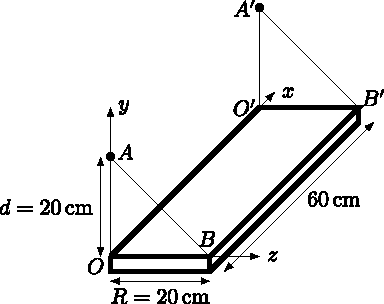
\includegraphics[width=\linewidth]{etg_plain.pdf}
		\end{center}
	\end{minipage}
}

\QR{%
	Exprimer les 4 forces de tension des câbles en fonction de normes arbitraires,
	la force de réaction $\Rf_N$ du mur sur la planche lorsque l'étagère est posée
	et en équilibre ainsi que le poids de l'étagère. $\Rf_N$ est supposée normale
	au mur. Calculer les valeurs numériques des normes des forces à l'aide de
	l'équilibre.
}{%
	On fait un schéma~:
	\begin{center}
		\includegraphics[width=.65\linewidth]{etg_corr}
	\end{center}
	\begin{itemize}
		\bitem{BdF}~:
		\begin{itemize}
			\item En B et B', les tensions des câbles obliques sont portées par les
			      vecteurs $\vvr{BA}$ et $\vvr{B'A'}$. Elles ont la même norme $T_1$
			      par symétrie, et on peut déduire les angles $\widehat{\rm OBA} =
				      \ang{45} = \widehat{\rm O'B'A'}$ puisque les triangles sont isocèles
			      et rectangles. Ainsi, avec $\cos(\ang{45}) = \frac{\sqrt{2}}{2} =
				      \sin(\ang{45})$, on trouve
			      \[
				      \Tf\ind{B} = \frac{\sqrt{2}}{2}T_1(\uy-\uz) = \Tf\ind{B'}
			      \]
			\item
			      En O et O', les tensions sont égales et verticales, soit
			      \[
				      \Tf\ind{O} = T_2 \uy = \Tf\ind{O'}
			      \]
			\item
			      De plus, la réaction du mur est $\Rf_N = R_N \uz$.
			\item Enfin, le poids s'exprime $\Pf = -mg\uy$
		\end{itemize}
		\bitem{BdM}~:
		\begin{itemize}
			\item le moment des tensions en B et B' se trouvent par le bras de
			      levier. Avec $H$ le projeté orthogonal de O sur AB, on trouve ${\rm
						      OH} = R \frac{\sqrt{2}}{2}$ (OBA triangle rectangle isocèle, OH
			      moitié de la diagonale et diagonale d'un carré de côté $a = a
				      \sqrt{2}$). Ainsi,
			      \begin{gather*}
				      \Mc_{\D}(\Tf\ind{B}+\Tf\ind{B'}) =
				      2 \times \Mc_{\D}(\Tf\ind{B}) =
				      \underbracket[1pt]{-}_{\mathclap{\text{sens direct}}}
				      2\,\,{\rm OH} \norm{\Tf\ind{B}}
				      \Lra
				      \Mc_{\D}(\Tf\ind{B}+\Tf\ind{B'}) = -2
				      \xunderbracket{R\frac{\sqrt{2}}{2}}_{\rm OH}
				      \xunderbracket{T_1}_{\norm{\Tf\ind{B}}}
				      \\\Lra
				      \boxed{\Mc_{\D}(\Tf\ind{B}+\Tf\ind{B'}) = -RT_1\sqrt{2}}
			      \end{gather*}
			\item Les moments des tensions $\Tf\ind{O}$ et $\Tf\ind{O'}$ ainsi que la
			      réaction du support $\Rf_N$ sont tous nuls, puisque leurs droites
			      d'actions passent par l'axe $\D$.
			\item Finalement, à l'équilibre la droite d'action du poids est à une
			      distance $R/2$ de l'axe de rotation, et comme le poids fait tourner
			      l'étagère dans le sens horaire, on a
			      \[
				      \Mc_{\D}(\Pf) = \frac{mgR}{2}
			      \]
		\end{itemize}
		\bitem{PFD}~: à l'équilibre, la somme des forces est nulle, soit
		\[
			\left\{
			\begin{array}{rlc}
				T_1 \sqrt{2} + 2T_2 & = mg  & \quad \text{sur}~\uy
				\\
				T_1 \sqrt{2}        & = R_N & \quad \text{sur}~\uz
			\end{array}
			\right.
		\]
		\bitem{TMC}~: à l'équilibre, il n'y a pas de rotation donc la somme des
		moments est nulle~:
		\[
			R T_1\sqrt{2} = \frac{mgR}{2}
		\]
		\bitem{Ccl}~: on trouve
		\[
			\boxed{T_1 = \frac{mg}{2 \sqrt{2}}} \Ra \xul{T_1 = \SI{3.5}{N}}
			\quad ; \quad
			\boxed{R_N = \frac{mg}{2}} \Ra \xul{R_N = \SI{4.9}{N}}
			\quad ; \quad
			\boxed{T_2 = \frac{mg}{4}} \Ra \xul{T_2 = \SI{2.5}{N}}
		\]
	\end{itemize}
}
\QR{%
	On imagine que les 2 câbles fixés en B et B' se rompent en même temps. La
	planche n'est alors retenue que par les câbles OA et OA', et elle tourne donc
	autour de l'axe $\D = (\rm OO')$. Nous négligerons son épaisseur et
	admettrons que son moment d'inertie par rapport à l'axe $\D$ vaut $J_{\D} =
		mR^2$. Montrer qu'alors~:
	\[
		\tp^2 = \frac{mgR}{J_{\D}}\sin(\th)
	\]
	En déduire la vitesse angulaire de la planche lorsqu'elle percute le mur.
}{%
	On reconnaît l'énergie cinétique dans la partie gauche de l'équation proposée.
	Il serait donc logique de partir du TEC. On sait que la puissance d'une force
	de rotation est $\Mc_{\D}(\Ff)\w$, donc le travail élémentaire associé est
	$\Mc_{\D}(\Ff)\dd{\th}$. Or, les tensions en B et B' n'existent plus et les
	moments des tensions en O et de la réaction normale sont toujours nuls~: il ne
	reste que le moment du poids.
	\smallbreak
	Or, avec un angle $\th$, le bras de levier diminue et on trouve $\Mc_{\D}(\Pf)
		= \frac{mgR}{2}\cos(\th)$. Ainsi,
	\begin{DispWithArrows*}
		\D\Ec_c &= W(\Pf)
		\Arrow{$\Ec_{c, \rm rot} = \frac{1}{2}J_{\D}\tp^2$\\
		$\Mc_{\D}(\Pf) = \frac{mgR}{2}\cos(\th)$}
		\\\Lra
		\frac{1}{2}J_{\D}\tp^2 &= \int_{0}^{\th}\frac{mgR}{2}\cos(\th)\dd{\th}
		\Arrow{$\int_0^{\th}\cos(\th)\dd{\th} = [\sin(\th)]_0^{\th}$\\$\sin(0)=0$}
		\\\Lra
		\frac{1}{2}J_{\D}\tp^2 &= \frac{mgR}{2}\sin(\th)
		\\\Lra
		\Aboxed{\tp^2 &= \frac{mgR}{J_{\D}}\sin(\th)}
		\qed
	\end{DispWithArrows*}
	Quand l'étagère touche le mur, $\th = \frac{\pi}{2}$, d'où
	\[
		\boxed{\tp_f = \sqrt{\frac{3g}{R}}}
		\Lra
		\xul{\tp_f = \SI{12}{rad.s^{-1}}}
	\]
}

\resetQ
\section{Entraînement par frottements}
\enonce{%
	\noindent
	\begin{minipage}[c]{.70\linewidth}
		On considère le système de deux disques en rotation, de moments d'inertie
		$J_1$ et $J_2$ par rapport à l'axe horizontal orienté par $\uz$. Ils sont tous
		les deux en liaison pivot parfaite. Le second disque a une vitesse angulaire
		$\w_0$, alors que le premier est initialement immobile. On translate
		lentement les disques le long de l'axe jusqu'à ce qu'ils rentrent en contact.
		Il n'y a plus de frottement après la mise en contact.
	\end{minipage}
	\hfill
	\begin{minipage}[c]{.30\linewidth}
		~
		\begin{center}
			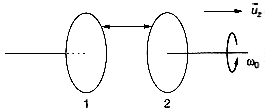
\includegraphics[width=\linewidth]{entr_frott-plain-white}
		\end{center}
	\end{minipage}
}
\QR{%
	À quelle condition sur les vitesses angulaires n'y a-t-il plus de
	frottements~? Déterminer alors les vitesses angulaires finales de deux disques
	par application du TMC sur le système total.
}{%
	Il n'y a plus de frottements si les deux disques vont à la même vitesse
	angulaire. Or, le moment cinétique \textbf{total} se conserve puisque
	$\Mc_{z}(\Pf_1) = \Mc_z(\Pf_2) = 0$ (forces passent par l'axe de rotation) et
	les liaisons pivot sont supposées parfaites~; ainsi $\dv{\Lc_z(\Sc)}{t} = 0$
	soit $\boxed{\Lc_z(\Sc) = \cte}$.
	\smallbreak
	En prenant une situation avant contact et à la fin du contact, on obtient
	\begin{DispWithArrows*}
		0 + J_2\w_0 &= J_1\w_{1,f} + J_2\w_{2,f}
		\Arrow{$\w_{1,f} = \w_{2,f} = \w_f$}
		\\\Lra
		\Aboxed{\w_f &= \frac{J_2}{J_1 + J_2}\w_0}
	\end{DispWithArrows*}
	Ce résultat ne dépend aucunement du type de frottements~; seule la durée du
	régime transitoire est impactée par l'expression des frottements.
}
\QR{%
	Faire un bilan d'énergie pour chaque disque séparément.
}{%
	Avec l'énergie potentielle de pesanteur prise à 0, on a~:
	\begin{enumerate}
		\item $\Delta{\Ec_{m,1}} = \Delta{\Ec_{c,1}} = \frac{1}{2}J_1\w_f{}^2 - 0$
		      soit
		      \[
			      \boxed{\Delta{\Ec_{m,1}} = \frac{1}{2}J_1 \left(
				      \frac{J_2}{J_1+J_2} \right)^2\w_0{}^2 > 0}
		      \]
		      Le disque 1 gagne donc de l'énerie cinétique grâce aux frottements avec le
		      second disque.
		\item Pour le second,
		      \begin{gather*}
			      \Delta{\Ec_{m,2}} = \Delta{\Ec_{c,2}} = \frac{1}{2}J_2\w_f{}^2 -
			      \frac{1}{2}J_2\w_0{}^2
			      \\\text{Soit}
			      \boxed{
				      \Delta{\Ec_{m,2}} = \frac{1}{2}J_2 \left( \left( \frac{J_2}{J_1+J_2}
					      \right)^2 - 1 \right)\w_0{}^2 < 0
			      }
		      \end{gather*}
		      Évidemment, le second \textbf{perd} de l'énergie~: il l'a cédée au premier
		      et perdu une partie par frottements.
	\end{enumerate}
}
\QR{%
	Faire le même bilan pour le système total.
}{%
	On somme les résultats précédents~:
	\begin{align*}
		\Delta{\Ec_m} & = \Delta{\Ec_{m,1}} + \Delta{\Ec_{m,2}}
		\\
		              & = \frac{1}{2} (J_1+J_2) \frac{J_2{}^2}{(J_1+J_2)^2}\w_0{}^2 -
		\frac{1}{2}J_2\w_0{}^2
		\\\Lra
		\Delta{\Ec_m} & = - \frac{1}{2}\frac{J_1J_2}{J_1+J_2}\w_0{}^2 < 0
	\end{align*}
}
\QR{%
	Commenter les résultats.
}{%
	À cause des frottements, l'énergie mécanique totale diminue. En revanche,
	l'énergie mécanique d'un sous-système peut augmenter ou diminuer.
}

\resetQ
\section{Expérience de \textsc{Cavendish}}
\enonce{%
	L'expérience réalisée par \textsc{Cavendish} en 1789 a permis à ce dernier
	d'obtenir une valeur remarquable de la constante de gravitation universelle,
	$\Gc$. Le dispositif est constitué de deux petites sphères, de masse $m =
		\SI{0.72}{kg}$, fixées aux extrémités d'une tige de masse négligeable, rigide,
	et longueur $\ell = \SI{180}{cm}$ et suspendue horizontalement, en son milieu, à
	un fil de torsion vertical et très fin de constante de torsion $C$~: si la tige
	tourne d'un angle $\th$ par rapport à sa position d'équilibre $\th = 0$, le fil
	exercice ainsi le couple de rappel $\vv{\G} = -C\th \uz$ sur la tige.
	\smallbreak
	Deux boules de plomb de masse $M = \SI{160}{kg}$ sont fixées, l'une derrière une
	petite sphère et l'autre devant l'autre petite sphère, à une distance $r =
		\SI{20}{cm}$ définie sur le schéma ci-dessous. Les deux forces d'attraction
	gravitationnelle produisent un couple qui fait tourner la tige d'un angle $\th$
	par rapport à sa position au repos. Les deux petites sphères se rapprochent
	ainsi des boules de plomb jusqu'à ce que la torsion du fil s'équilibre avec le
	couple gravitationnel.
	\begin{figure}[htbp!]
		\centering
		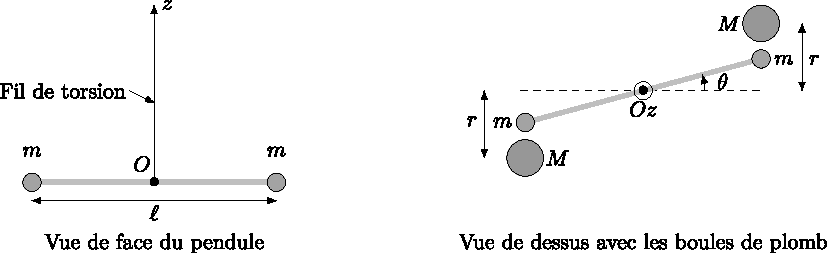
\includegraphics[width=.8\linewidth]{cav_plain}
	\end{figure}
}

\begin{blocQR}
	\item Nous cherchons dans un premier temps à déterminer la constante de
	torsion $C$ du pendule en faisant osciller celui-ci. Les boules en plomb ne
	sont pas encore présentes.
	\QR{%
		Montrer à l'aide du TMC que l'oscillateur est harmonique, de pulsation
		propre $\w_0 = \sqrt{\frac{2C}{m \ell^2}}$.
	}{%
		Soit $\Delta = (\Or z)$ l'axe vertical ascendant. Chacune des deux sphères
		étant en mouvement de rotation de rayon $\ell/2$ autour de $\Delta$ à la
		même vitesse angulaire $\tp$ et la masse de la tige étant négligée, le
		moment cinétique total de l'ensemble \{tige+deux sphères\} par rapport à
		$\Delta$ est $\Lc_{\D} = \frac{m \ell^2}{2}\tp$.
		\smallbreak
		Ce système est soumis à l'action de son poids et de la tension du fil, dont
		les moments par rapport à $\D$ sont nuls, et au couple de torsion $\vv{\G} =
			-C\th \uz$.
		\smallbreak
		L'application du TMC scalaire conduit donc à
		\begin{align*}
			\frac{m \ell^2}{2}\tpp                & = -C\th
			\\\Lra
			\Aboxed{\tpp + \frac{2C}{m \ell^2}\th & = 0}
		\end{align*}
		C'est bien un oscillateur harmonique de pulsation $\w_0 = \sqrt{\frac{2C}{m
					\ell_2}}$.
	}
	\QR{%
	La mesure de la période $T_0$ des oscillations donne $T_0 =
		\SI{7.0}{min}$. En déduire la valeur de $C$.
	}{%
	\[
		\boxed{C = \frac{2\pi^2 m \ell^2}{T_0{}^2}}
		\Ra
		\xul{C = \SI{2.6e-4}{N.m.rad^{-1}}}
	\]
	}
\end{blocQR}
\QR{%
	Les boules étant placées, déterminer l'expression de la déviation angulaire
	$\th$ par rapport à la position d'équilibre. On tiendra compte du fait que
	$\th$ est extrêmement faible pour évaluer le couple exercé par les deux
	boules de plomb.
}{%
	On se place dans le système de coordonnées polaires, de base associée
	$(\ur,\ut,\uz)$ pour chacune des deux sphères, et on estime que la distance
	entre une des sphères et la boule correspondante est
	\[
		r - \frac{\ell}{2}\sin(\th) \approx r - \frac{\ell}{2}\th
	\]
	On néglige aussi l'action de la boule la plus éloignée. On suppose de plus que
	la force de gravitation exercée par la boule sur la sphère est portée par
	$\ut$, et on utilise le développement limité $(1-x)^{-2} \Sim_{x \to 0}
		1+2x$~:
	\[
		\Ff_g =
		\Gc\frac{mM}{\left( r - \frac{\ell}{2}\th \right)^2}\ut \approx
		\frac{\Gc mM}{r^2}\left( 1 + \frac{\ell}{r}\th \right)\ut
	\]
	Le moment de cette force par rapport à $\Delta$ est ainsi, avec $d$ du bras de
	levier égal à $\ell/2$~:
	\[
		\Mc_{\D}(\Ff_g) = \frac{\Gc mM \ell}{2r^2} \left( 1+\frac{\ell}{r}\th \right)
	\]
	On en déduit que le moment total des deux forces gravitationnelles est le
	double de ce moment unique~:
	\begin{DispWithArrows*}[]
		\Mc_{\D}(\Ff_{g,\tot}) &= \frac{\Gc mM \ell}{r^2} \left( 1+\frac{\ell}{r}\th \right)
		\shortintertext{Ainsi, avec le TMC~:}
		\frac{m \ell^2}{2}\tpp &=
		-C\th + \frac{\Gc mM \ell}{r^2} \left( 1+\frac{\ell}{r}\th \right)
		\Arrow{Équilibre}
		\\\Ra
		\Aboxed{\th\ind{eq} &= \frac{\Gc mM \ell r}{Cr^3 - \Gc mM \ell_2}}
	\end{DispWithArrows*}
}
\QR{%
La valeur obtenue par \textsc{Cavendish} à l'aide de ce dispositif et $\Gc =
	\SI{6.75e-11}{N.m^2.kg^{-2}}$. En déduire la déviation angulaire et commenter.
}{%
\[
	\xul{\th\ind{eq} = \SI{1.4e-3}{rad}}
\]
Ainsi, \textsc{Cavendish} avait donc développé une méthode de mesure d'angle
avec une précision inférieure au milliradian~!
\smallbreak
Pour une vidéo sur le sujet, voir notamment celle de Steve \textsc{Mould}~:
\url{https://youtu.be/70-_GBymrck?si=6iBDUeYnSixdLS3c}
}

\end{document}
